\documentclass[12pt,mathserif]{beamer}
\usetheme{Madrid}
\usecolortheme{}
\setbeamertemplate{caption}[numbered] %нумерация заголовков

\setbeamertemplate{navigation symbols}{}
\usefonttheme{serif}
\useinnertheme{circles}
\usepackage{cmap}
\usepackage[utf8]{inputenc}
\usepackage[OT1]{fontenc}
\usepackage[english, russian]{babel}
%Математика
\usepackage{amsmath}
\usepackage{amssymb}
\usepackage{mathtext}
\usepackage{mathrsfs}
\usepackage{amscd}
\usepackage{onlyamsmath}
\usepackage{bm}

\usepackage{graphicx}
\usepackage{indentfirst}
\usepackage{fancyvrb}

\bibliographystyle{gost2008}
\usepackage{hyperref}
\usepackage{xcolor}
\usepackage[labelfont={color=black}]{caption} %цвет заголовков
\definecolor{linkcolor}{HTML}{799B03} % цвет ссылок
\definecolor{urlcolor}{HTML}{799B03} % цвет гиперссылок

\hypersetup{pdfstartview=FitH,  linkcolor=linkcolor,urlcolor=urlcolor, colorlinks=true}

\makeatletter
\newcommand\titlegraphicii[1]{\def\inserttitlegraphicii{#1}}
\titlegraphicii{}
%Шаблон титульного слайда
\setbeamertemplate{title page}
{
	{\usebeamercolor[fg]{titlegraphic}\inserttitlegraphic\hfill\inserttitlegraphicii\par}
	\begin{centering}
		\begin{beamercolorbox}[sep=8pt,center]{institute}
			\usebeamerfont{institute}\insertinstitute
		\end{beamercolorbox}
		\begin{beamercolorbox}[sep=4pt,center]{title}
			\usebeamerfont{title}\inserttitle\par%
			\ifx\insertsubtitle\@empty%
			\else%
			\vskip0.25em%
			{\usebeamerfont{subtitle}\usebeamercolor[fg]{subtitle}\insertsubtitle\par}%
			\fi%     
		\end{beamercolorbox}%
		\vskip1em\par
		\begin{beamercolorbox}[sep=5pt,center]{date}
			\usebeamerfont{date}\insertdate
		\end{beamercolorbox}%\vskip0.5em
		\begin{beamercolorbox}[sep=1pt,left]{author}
			\usebeamerfont{author}\insertauthor
		\end{beamercolorbox}
	\end{centering}
	%\vfill
}


%Создание титульного слайда
\makeatother
\author[Чесаков\,М.\,Е.]{Выполнил студент 221 группы факультета КНиИТ \\ \textit{Чесаков Максим Евгеньевич}}

\title[Курсовая работа]{\large Аналитические методы в теории телетрафика}

%\subtitle{Вариант \textnumero 1}

\institute[]{\footnotesize Саратовский национальный исследовательский государственный университет имени Н.\,Г.\,Чернышевского \\ 
\vskip0.35em%
Кафедра системного анализа и автоматического управления

~\

}
\date{}

\begin{document}
	
	\begin{frame}[plain]
	\maketitle

	\begin{flushleft}
		Научный руководитель: \\
		доцент, к.\,ф.-м.\,н.  \textit{Станкевич Елена Петровна}
	\end{flushleft}

\end{frame}
	
	\begin{frame}
		\frametitle{Телетрафик}
		Интенсивность трафика – среднее число ресурсов, занятых обслуживанием трафика:
		\[
		\overline{A}(t_1,t_2) = \frac{1}{t_2 - t_1}\int\limits_{t_1}^{t_2} A(t) \, dt ,
		\]
		где $A(t)$ --- число занятых обслуживанием ресурсов в каждый момент времени.
		Единица измерения --- эрланг.

		Скорость поступления сообщений $\lambda = \displaystyle\frac{n}{T}$.
	\end{frame}

	\begin{frame}
		\frametitle{Система M/M/1}
		\begin{figure}
			\centering
			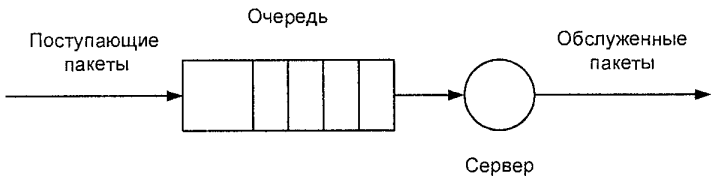
\includegraphics[width=11.7cm]{ris4.png}
		\end{figure}
		
		$\mu$ --- скорость обработки пакетов.
		
		$\rho = \displaystyle\frac{\lambda}{\mu}$. ~ $\rho < 1$ --- условие стационарности.		
	\end{frame}

	\begin{frame}
		\frametitle{Система M/M/1}
		\begin{equation}
			p_k = p_0 \left( \frac{\lambda}{\mu} \right)^k; k \geq 0,
		\end{equation}
		\begin{equation}
			p_0 = 1 - \rho,
		\end{equation}
		\begin{equation}
			p_k = (1-\rho)\rho^k,~k \geq 0,
		\end{equation}
		\begin{equation}
			\overline{N} = \sum_{k=0}^{\infty} kp_k = (1 - \rho) \sum_{k=0}^{\infty} k\rho^k = \frac{\rho}{1 - \rho},
		\end{equation}
		\begin{equation}
    		T = \frac{\overline{N}}{\lambda} = \left(\frac{\rho}{1-\rho}\right)\left(\frac{1}{\lambda}\right) = \frac{1}{\mu(1-\rho)} = \frac{1}{\mu - \lambda},
		\end{equation}
		\begin{equation}
    		\overline{N_q} = \overline{N} - \rho = \frac{\rho^2}{1-\rho},
		\end{equation}
		\begin{equation}
			\overline{W} = \frac{1}{\lambda} \overline{N_q} = \frac{\rho}{\mu(1-\rho)}=T\rho.
		\end{equation}
	\end{frame}
	
	\begin{frame}
		\frametitle{Графики зависимостей характеристик от $\lambda$}
		\begin{figure}
			\centering
			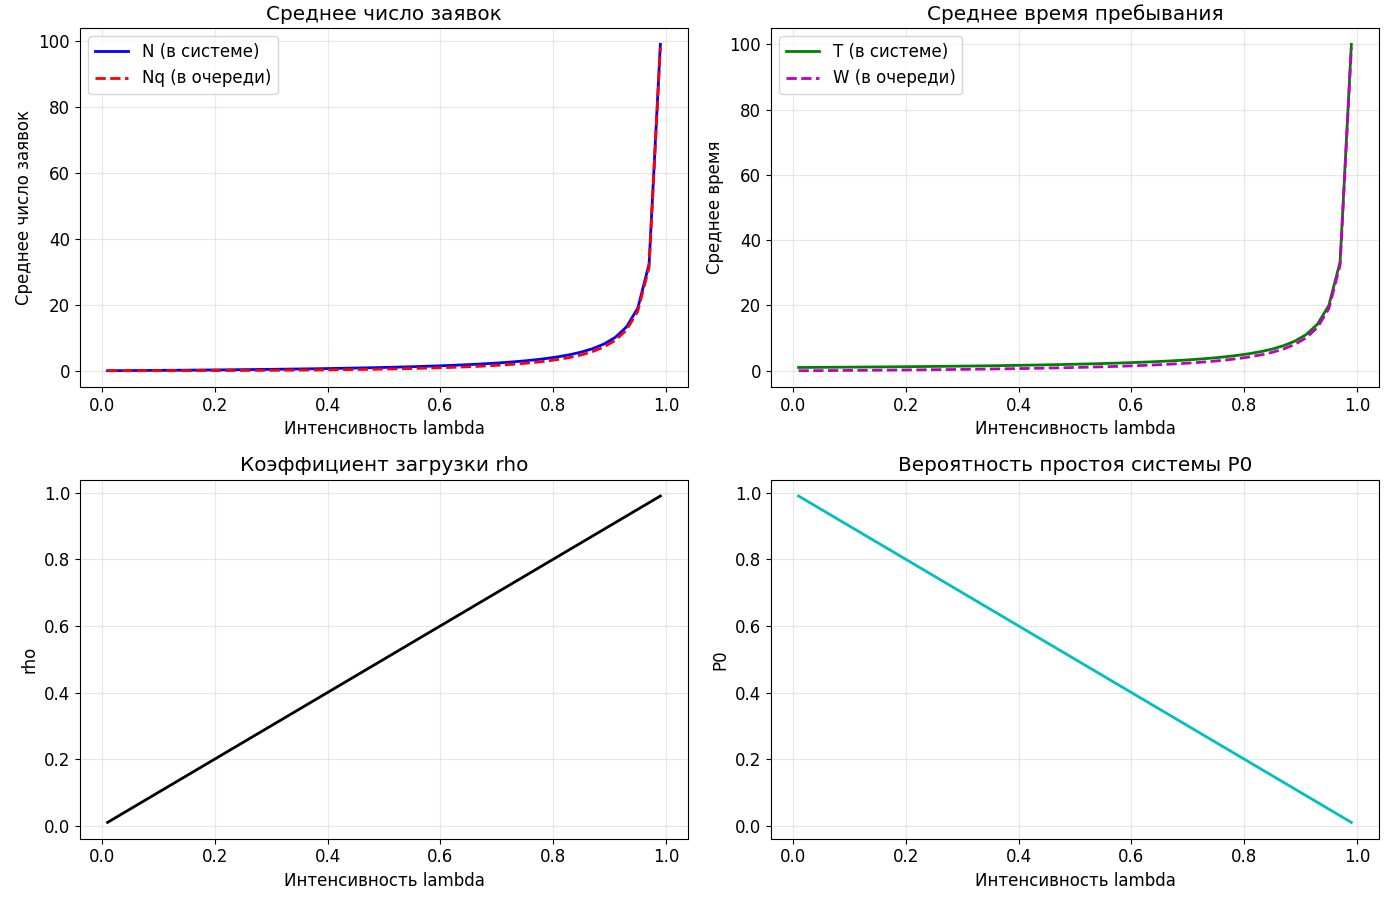
\includegraphics[width=11.7cm]{ris11.png}
		\end{figure}
	\end{frame}
	
	\begin{frame}
		\frametitle{Графики зависимостей характеристик от $\mu$}
		\begin{figure}
			\centering
			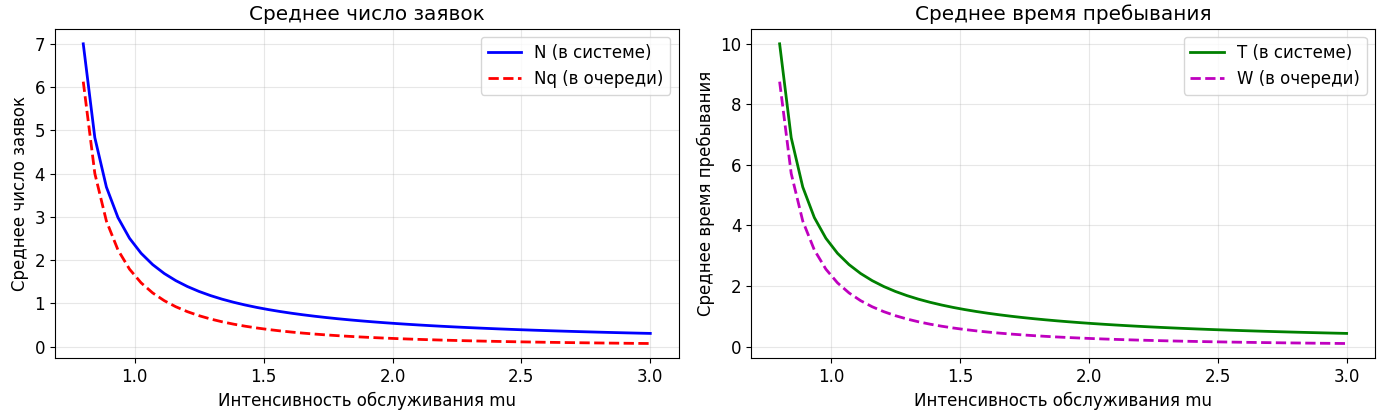
\includegraphics[width=11.7cm]{ris12.png}
		\end{figure}
	\end{frame}
	
	\begin{frame}
		\frametitle{\large
			Стационарное распределение вероятностей состояний}
		\begin{figure}
			\centering
			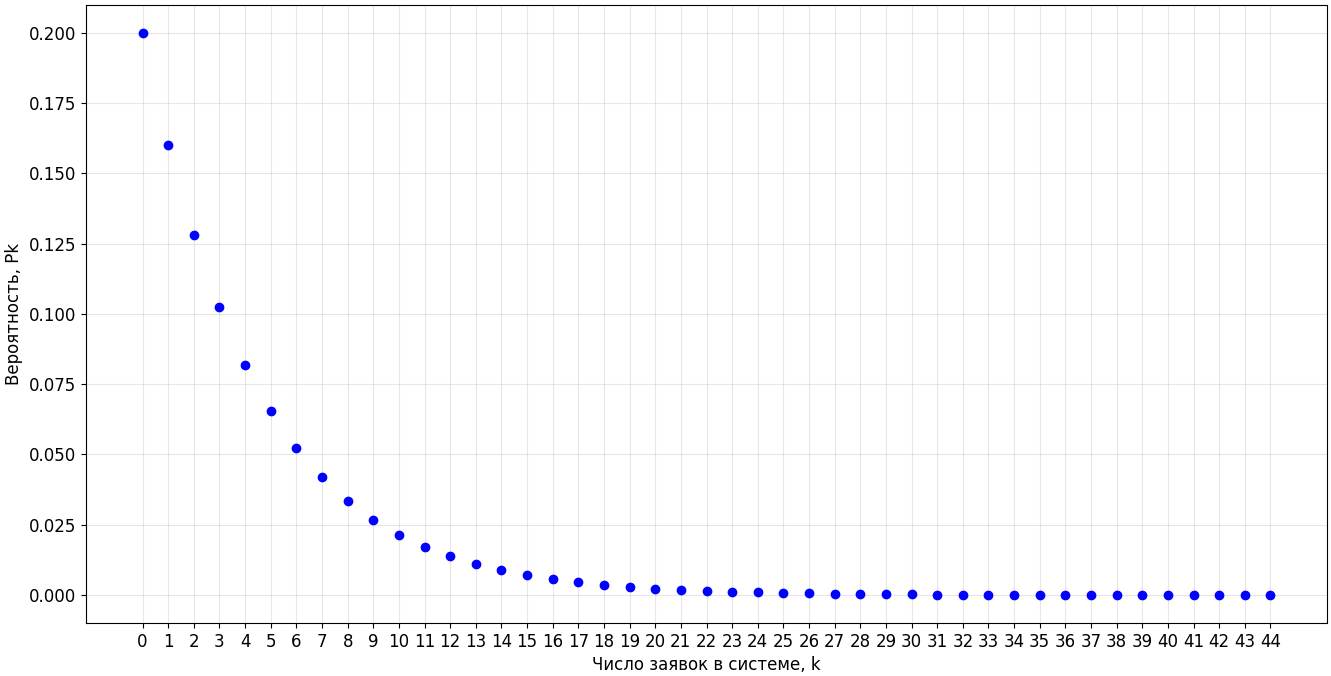
\includegraphics[width=11.7cm]{ris13_new_new.png}
		\end{figure}
	\end{frame}
	
	\begin{frame}

		\vspace*{1cm}
		\centering
		\Large
		{\sc Спасибо за внимание!}
	
    \end{frame}
	
\end{document}